\documentclass[conference]{IEEEtran}
\IEEEoverridecommandlockouts
% The preceding line is only needed to identify funding in the first footnote. If that is unneeded, please comment it out.
\usepackage{cite}
\usepackage{amsmath,amssymb,amsfonts}
\usepackage{algorithmic}
\usepackage{graphicx}
\usepackage{textcomp}
%%% GLOSSARIES
\usepackage{glossaries}

\makeglossaries

\newacronym{tls}{TLS}{Transport Layer Security}%
\newacronym{ssl}{SSL}{Secure Sockets Layer}%
\newacronym{ietf}{IETF}{Internet Engineering Task Force}%
\newacronym{mac}{MAC}{Message Authentication Code}%
\newacronym{psk}{PSK}{Pre-Shared Key}%
\newacronym{rpk}{RPK}{Raw Public Key}%
\newacronym{aead}{AEAD}{Authenticated Encryption With Associated Data}%
\newacronym{pkc}{PKC}{Public Key Cryptography}%
\newacronym{hkdf}{HKDF}{HMAC-based Extract-and-Expand Key Derivation Function}%
\newacronym{html}{HTML}{Hypertext Markup Language}%
\newacronym{https}{HTTPS}{Hypertext Transfer Protocol Secure}%
\newacronym{ecc}{ECC}{Elliptic Curve Cryptography}%
\newacronym{iv}{IV}{Initialization Vector}%
\newacronym{ecdh}{ECDH}{Elliptic Curve Diffie-Hellman}%
\newacronym{ecdhe}{ECDHE}{Elliptic Curve Diffie-Hellman Ephemeral}%
\newacronym{ecdsa}{ECDSA}{Elliptic Curve Digital Signature Algorithm}%
\newacronym{rfc}{RFC}{Request For Comment}%
\newacronym{prf}{PRF}{Pseudo-Random Function}%
\newacronym{rsa}{RSA}{Rivest-Shamir-Adleman}%
\newacronym{dh}{DH}{Diffie-Hellman}%
\newacronym{pms}{PMS}{premaster secret}%
\newacronym{dsa}{DSA}{Digital Signature Algorithm}%
\newacronym{pfs}{PFS}{Perfect Forward Secrecy}%
\newacronym{mitm}{MITM}{Man In The Middle}%
\newacronym{ac}{AC}{Asymmetrical Cryptography}%
\newacronym{sc}{SC}{Symmetrical Cryptography}%
\newacronym{iot}{IoT}{Internet Of Things}%
\newacronym{dtls}{DTLS}{Datagram TLS}%
\newacronym{coap}{CoAP}{Constrained Application Protocol}%
\newacronym{ec}{EC}{Elliptic Curve}%
\newacronym{sca}{SCA}{Side-Channel Attack}%
\newacronym{ocsp}{OCSP}{Online Certificate Status Protocol}
\newacronym{crl}{CRL}{Certificate Revocation List}
\newacronym{ca}{CA}{Certification Authority}
\newacronym{sni}{SNI}{Server Name Indication}
\newacronym{dos}{DoS}{Denial-of-Service}
\newacronym{ddos}{DDoS}{Distributed Denial-Of-Service}
\newacronym{pki}{PKI}{Public Key Infrastructure}
\newacronym{ae}{AE}{Authenticated Encryption}
\newacronym{nsa}{NSA}{US National Security Agency}
\newacronym{apk}{APK}{Authorized Public Key}


\def\BibTeX{{\rm B\kern-.05em{\sc i\kern-.025em b}\kern-.08em
    T\kern-.1667em\lower.7ex\hbox{E}\kern-.125emX}}
\begin{document}

\title{TLS For IoT}

\author{\IEEEauthorblockN{Illya Gerasymchuk}
\IEEEauthorblockA{\textit{Instituto Superior Tecnico} \\
Lisbon, Portugal \\
illya@iluxonchik.me}
}

\maketitle

\begin{abstract}
\gls{tls} is, one of the most used communication security protocols, it is however, not suitable in the context of \gls{iot}. The resource-limited nature
of a big part of \gls{iot} devices does not allow for the use of computationally complex
and memory demanding operations present in a standard \gls{tls} implementation. Most of previous work focused entirely on \gls{dtls} and
can not be easily integrated with existing deployments. This work focuses on
how \gls{tls} and the extension mechanism can be used to define a framework
to adapt the protocol to specific needs. This is the approach that
will be followed in the second part of the work. Having an adaptable and
easy to use solution is crucial for its adaptation in \gls{iot},
where security might have been completely foregone otherwise.
\end{abstract}

\begin{IEEEkeywords}
TLS, DTLS, SSL, IoT, cryptography, protocol, lightweight cryptography
\end{IEEEkeywords}

\section{Introduction}
The Internet of Things (IoT) is a network of devices, from simple sensors to smartphones and wearables
which are connected together. In fact, it can be any other object that has an assigned
IP address and is provided with the ability to transfer data over a network. Even a salt shaker\cite{SMALTThe76:online} can now be part of the global network.

The \gls{iot} technology provides many benefits, from personal comfort to
transforming entire industries, mainly due to increased connectivity and
new sources for data analysis. The technological development, however, tends to focus on
innovative design rather than on privacy and security. \gls{iot} devices frequently
connect to networks using inadequate security and are hard to update when
vulnerabilities are found.

This lack of security in the \gls{iot} ecosystem has been exploited by the
the \textit{Mirai} botnet\cite{sec17ant94:online} when it overwhelmed several high-profile
targets with massive \gls{ddos} attacks. This is the most devastating attack involving \gls{iot}
devices done to date. However, the \textit{Reaper} botnet\cite{ReaperCa10:online} could be
even worse if it is ever put to malicious use. Similar attacks will inadvertently
come in the future.

\gls{tls} is one of the most used security protocols in the world, allowing two peers
to communicate securely. It is designed to run on top of a reliable, connection-oriented
protocol, such as TCP. Datagram TLS (DTLS) is the version of \gls{tls} that runs on top
of an unreliable transport protocol, such as UDP. Most \gls{iot} devices have
very limited processing power, storage and energy. Moreover, the performance of
TCP is known to be inefficient in wireless networks, due to its congestion control
algorithm. This situation is worsened with the use of low-power radios and lossy
links found in sensor networks. Therefore, the use of TCP with \gls{iot}
is usually not the best option. For this reason, \gls{dtls}, which runs on top
of UDP, is used more frequently in such devices. The work that will be done in the context of this dissertation, can however,
be applied to either one of them, so even though mostly
\gls{tls} will be mentioned, almost everything can also be applied to \gls{dtls}. This is a consequence of \gls{dtls} being just an adaption of \gls{tls} over unreliable transport protocols, with no changes done to
the core protocol.

The problem in using (D)\gls{tls} in \gls{iot} is that it is not lightweight, since
it has not been designed for such environments. An \gls{iot} device may only have
$256$ KB of RAM and needs to conserve the battery, while sending and receiving
a large amount of small information constantly. For example, consider the case of a temperature sensor
that sends temperature measures every $30$ seconds to a server. In this case
it just needs to send a few bytes of data and do it with minimal overhead, to conserve
RAM and battery. If that sensor is going to use (D)\gls{tls} $1.2$, it will need
two extra roundtrips before it can send any data. This can result in an overhead of several hundreds of
milliseconds. Besides that, it will need to perform heavy mathematical operations
involved in cryptography, using even more energy and taking even more time.
Given this, there is a clear need for a more lightweight (D)\gls{tls} for the \gls{iot}. This is the problem that we will be addressing in this work.

In the process of the work on this dissertation, we have made several
contributions to the \gls{tls} $1.3$ specification \cite{PullRequ68:online}. Among
several contributions, we corrected some
inconsistencies/incompletenesses in the specification (e.g.
the document mentioned some extensions as being mandatory, yet they
were not present in the "Mandatory-to-Implement" section \cite{addmessa28:online}) and some parts of the specification that
were wrong, like the "Backwards Compatibility" section \cite{fixBackw47:online}. As a result, we were formally recognized as contributors and our name will be in the final document specifying the
\gls{tls} $1.3$ protocol. We are in no way affiliated with the
\gls{ietf} or any of the entities responsible for the development of
the \gls{tls} $1.3$ specification.

In our work, we are using the \textit{mbedTLS} library\cite{SSLLibra89:online}, which provides
a lightweight \gls{tls} implementation for the \gls{iot} devices.
In the process of profiling the library and studying its code, we
have identified two bugs. The first one is related to the use of
\textit{SHA-1}-signed certificates\cite{updatete80:online} in example
programs that come with \textit{mbedTLS}, which are not supported in the
default configuration. We have provided a fix for that issue\cite{updatete80:online}. The second bug is both: a deviation from the
\gls{tls} $1.2$ protocol specification and a security issue. The problem
is that ciphesuites that should only allow \textit{RSA}-signed certificates,
besides those, also allow \textit{ECDSA}-signed ones. We have reported the
issue and provided proof of concept code \cite{TLSECDHR77:online}.

The document is organized as follows: Section II describes the \gls{tls} protocol. Section III summarizes the related work. Section IV describes the goal of this work. In Section V, the work current work is outlined. Finally, the conclusion is done in Section VI.

\section{The \gls{tls} Protocol}

\gls{tls} is a \textbf{client-server} protocol
that runs on top a \textbf{connection-oriented and reliable transport protocol},
such as \textbf{TCP}. Its main goal is to provide \textbf{privacy} and \textbf{integrity}
between the two communicating peers. Privacy implies that a third party will not
be able to read the data, while integrity means that a third party will not be
able to alter the data.

In the TCP/IP Protocol Stack, \gls{tls} is placed between the \textbf{Transport}
and \textbf{Application} layers. It is designed to simplify the establishment
and use of secure communications from the application developer's standpoint.
The developer's task is reduced to creating a "secure" connection (\textit{i.e.} socket), instead of a "normal" one.

A secure communication established using \gls{tls} has two phases.

\begin{enumerate}
\item The communicating peers authenticate one to another and negotiate security parameters, such as the secret keys and the encryption algorithm. This occurs under the Handshake Protocol.
\item The communicating peers exchange cryptographically protected data
using the security parameters negotiated during the Handshake Protocol. This
occurs under the Record Protocol.
\end{enumerate}

In order to
achieve its goals, during the Handshake Protocol the client and the server
exchange various messages. The message flow is depicted in Figure \ref{fig:tls-12-handshake}. \codeword{*} indicates situation-dependent
messages that are not always sent.

\gls{tls} provides the following \textbf{security services}:
\begin{itemize}
\item \textbf{authentication} - both, \textbf{peer entity} and \textbf{data origin} (or \textbf{integrity})
authentication.
\subitem \textbf{peer entity authentication} - a peer has a guarantee that it is talking to certain entity, for example, \codeword{www.google.com}.
This is achieved thought the use of \gls{ac}, also known as \gls{pkc}, (\textit{e.g.} \codeword{RSA} and \codeword{DSA})
or \textbf{symmetric key cryptography}, using a \gls{psk}.
\item \textbf{confidentiality} - the data transmitted between the communicating
entities (the client and the server) is encrypted. Symmetric cryptography is
used for data encryption (\textit{e.g.}, \codeword{AES}).
\item \textbf{integrity} (also called \textbf{data origin authentication}) - a peer can be sure that the data was not modified or forged,
\textit{i.e.}, there is a guarantee that the received data is coming from the expected entity. For example, a peer can be sure
that the \codeword{index.html} file that was sent to when it connected to \codeword{www.google.com} did, in fact,
come from \codeword{www.google.com} and it was not tampered with by an attacker (\textbf{data integrity}). This is achieved either through the use
of a keyed \gls{mac} or an \gls{aead} cipher.
\item \textbf{replay protection} (also known as \textbf{freshness}) -
a peer can be sure that a message has not been replayed. This is
achieved through the use of sequence numbers. Each \gls{tls} record has a different sequence number, which is incremented. If a non-\gls{aead} cipher is used, the sequence number is a direct input of the \gls{mac} function. If an \gls{aead} cipher is used, a nonce derived from the sequence number is used as input to that cipher.
\item \textbf{perfect forward secrecy (PFS)} - the confidentiality of the past
interactions is preserved even if the long-term secret is compromised.
\end{itemize}

Despite using \gls{pkc}, \gls{tls} does \textbf{not} provide \textbf{non-repudiation services}:
neither \textbf{non-repudiation with proof of origin}, which addresses the peer denying
the sending of a message, nor \textbf{non-repudiation with proof of delivery}, which
addresses the peer denying the receipt of a message. This is due to the fact that
instead of using \textbf{digital signatures}, either a keyed \gls{mac} or an \gls{aead}
cipher is used, both of which require a secret to be \textbf{shared} between the peers.

It is not required to use all of the security services every situation.In this sense, \gls{tls} is like a framework that allows to select which security services should be used for a communication session. As an example,
certificate validation might be skipped, which means that the \textbf{authentication} guarantee is not provided. There are some differences regarding this claim between \gls{tls} $1.2$\cite{RFC5246}
and \gls{tls} $1.3$\cite{I-D.ietf-tls-tls13}. For example, while in the first there is a \codeword{null}
cipher (no authentication, no confidentiality, no integrity), in the latter
this is not true.

\begin{figure}
        \centering
        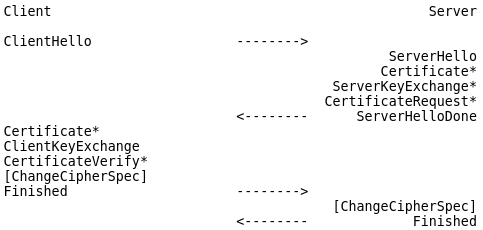
\includegraphics[width=0.5\textwidth]{../thesis/img/tls-12-full-handshake3.png} % first figure itself
        \caption{\label{fig:tls-12-handshake} \gls{tls} $1.2$ message flow for a full handshake}
\end{figure}


\section{Related Work}

Most of the work has been centered around \gls{dtls},
even though the majority of solutions can be applied to \gls{tls} as well.
Herein we want to further explore \gls{tls} optimization. There is clearly a need for that, specially with \gls{coap} over
TCP and \gls{tls} standard being currently developed\cite{I-D.ietf-core-coap-tcp-tls}. The mentioned standard does not explore any \gls{tls}
optimizations, and since any \gls{iot} device using it in the future would benefit from
them, this is an important area to explore. \gls{coap}\cite{RFC7959} is often
referred to as the "HTTP protocol for constrained devices".

None of the related work explored
(D)\gls{tls} 1.3, mainly because the protocol is still in draft stages, however, major design changes are not expected at this point.

The majority of the work done in the area proposes a solution that is either tied to a
specific protocol, such as \gls{coap}, or requires an introduction of a third-party
entity, such as the trust anchor in the case of the S3K system\cite{S3KScala62:online} or
even both. This has two main issues. First, a protocol-specific solution cannot
be easily used in an environment where (D)\gls{tls} is not used with that protocol. Second, the requirement of a third-party
introduces additional cost and complexity, which will be a big resistance factor
in adopting the technology. This is specially true for developers working on
personal projects or projects for small businesses, leaving the communications insecure
in the worse case scenario.

\section{Proposed Solution}

There is currently
no tool which can suggest a (D)\gls{tls} configuration, based
on the provided environment's limitations (e.g. available
memory, power, processing speed) and security requirements (e.g. PFS, data privacy). The solution will be fully \gls{tls} compatible,
since it will not modify any part of the protocol.

The goal of this work is to develop a framework that would
suggest a (D)\gls{tls} configuration based on the needs and
limitations of the environment. This configuration would
include key exchange algorithms, encryption algorithms
and \gls{tls} options (e.g. extensions), among others.

The solution will be developed for
(D)\gls{tls} version $1.2$, while also bearing in mind the new $1.3$ version.

To achieve this goal, a thorough evaluation of every part of (D)\gls{tls} is
needed. The main parts that will be evaluated are power consumption and the number CPU cycles used.

We would like to associate a quantitative
cost with every (D)\gls{tls} feature. For example, we would like to answer
questions such as \textit{"How much does Perfect Forward Secrecy cost, in terms of CPU cycles?"}.
This will help the application developers in making decisions related
to the security/performance trade off.

\section{Current Work}

In order to understand which features of (D)\gls{tls} should be
used, as an answer to the limitations and requirements of the context,
it's important to associate a cost (e.g. number of CPU cycles used) with each one of those features.
For this reason, we are currently working on profiling the various parts of the \gls{tls} protocol.

All of the evaluation work is being done on the \gls{tls} implementation of the \textit{mbedTLS} library\cite{SSLLibra13:online}.

\textit{mbedTLS} has various \gls{tls} configurations. Some of those
configurations are ciphersuites (key exchange algorithm + encryption function + hash function), others are protocol features (e.g.
session resumption, which allows to establish a connection using
less computing resources, by using constructs from a previously
established session), while others are extensions to the \gls{tls} protocol.

Currently, we are focused on profiling the
\gls{tls} ciphersuites. More specifically, we are profiling the
handshake portion of the protocol. After the handshake, the data
is exchanged using the negotiated encryption and hash functions,
as well as the associated secret keys. The latter is not
\gls{tls} specific and comes down to evaluating the performance of
various encryption and digest algorithms, which has already
been done in various works, such as \cite{kansal2014performance}
\cite{rihan2015performance} \cite{patil2016comprehensive} \cite{dahal2013performance}.

Therefore, we are currently focused on evaluating
the cost of various key exchange configurations. The chosen key
exchange determines various security properties of the communication,
namely the presence or absence of PFS and authentication guarantee.
Each one of those security services has an associated cost.

\textit{mbedTLS} comes with $161$ ciphersuites \cite{Supporte13:online}. Evaluating and analyzing the performance of each one manually would be very time consuming, if not impossible,
given the limited time available. The fact every ciphersuite can have
different configuration options (such as the certificates used and
the information contained in them) aggravates this issue even more.

For this reason, we developed an automated profiling tool \cite{iluxonch55:online}.
This tool runs a client/server connection for the provided list of
ciphersuites, collects the number of CPU cycles used by the user-specified
functions and presents the results in a graph. Using this tool, we were
able to evaluate all of the $161$ ciphersuites and reach some initial
conclusions.

The tool uses valgrind to profile the ciphersuites
and obtain the number of CPU cycles used by each one. It is important
to note that valgrind does not count the actual number of CPU
cycles used, but rather an estimate of them. All of the executrices
have been compiled, ran and profiled on an \textit{x86\_64 GNU/Linux} machine (Kernel \textit{4.15.13-1-ARCH}).

\begin{figure}
        \centering
        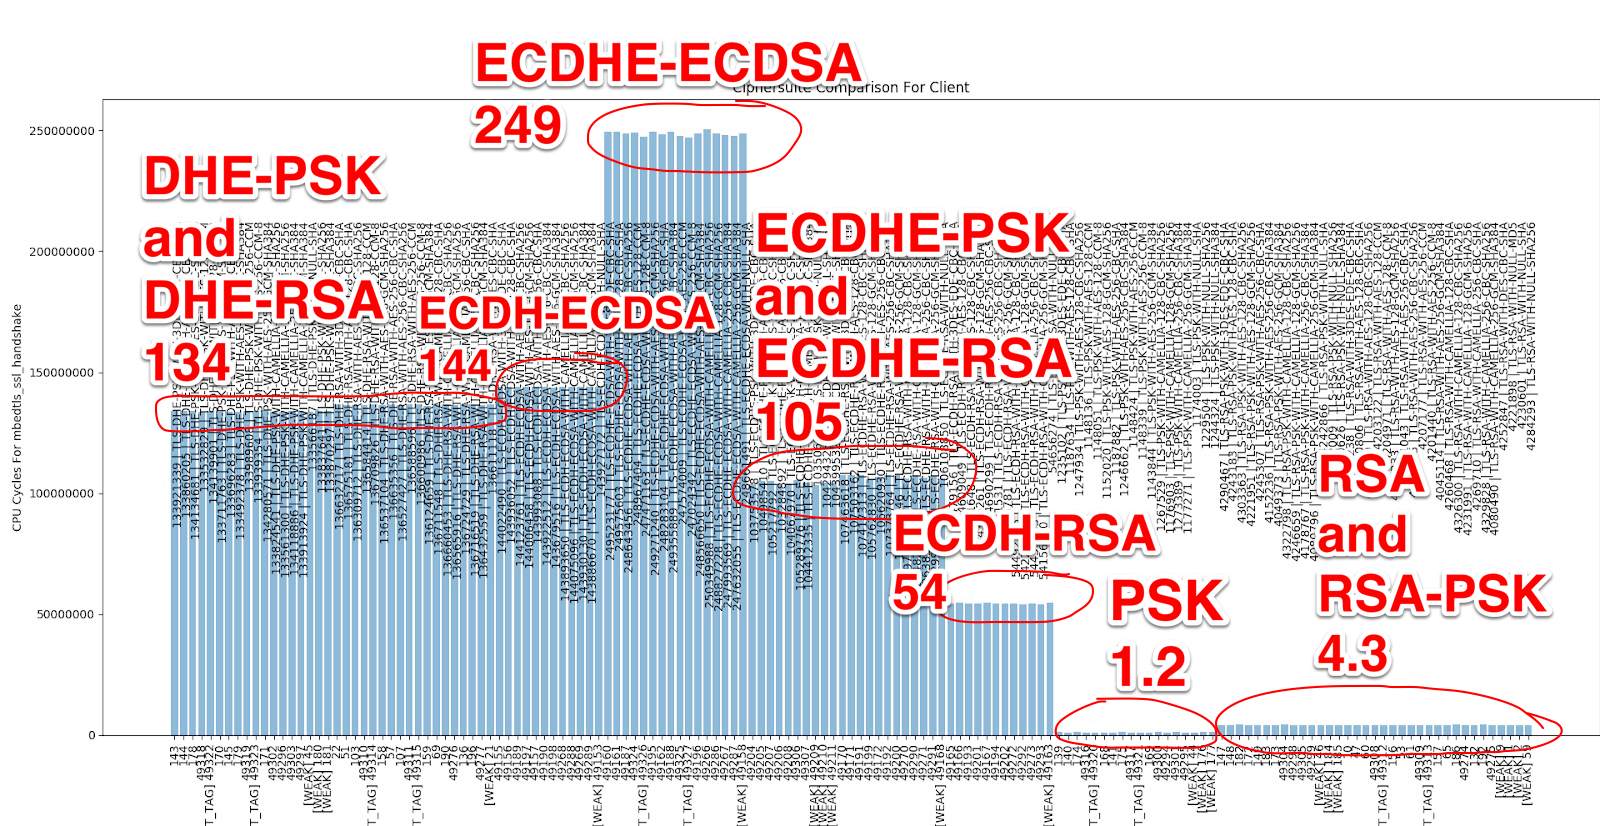
\includegraphics[width=0.5\textwidth]{./cli-graph.png} % first figure itself
        \caption{\label{fig:cligraph} Client ciphersuite profiling}
\end{figure}

\begin{figure}
        \centering
        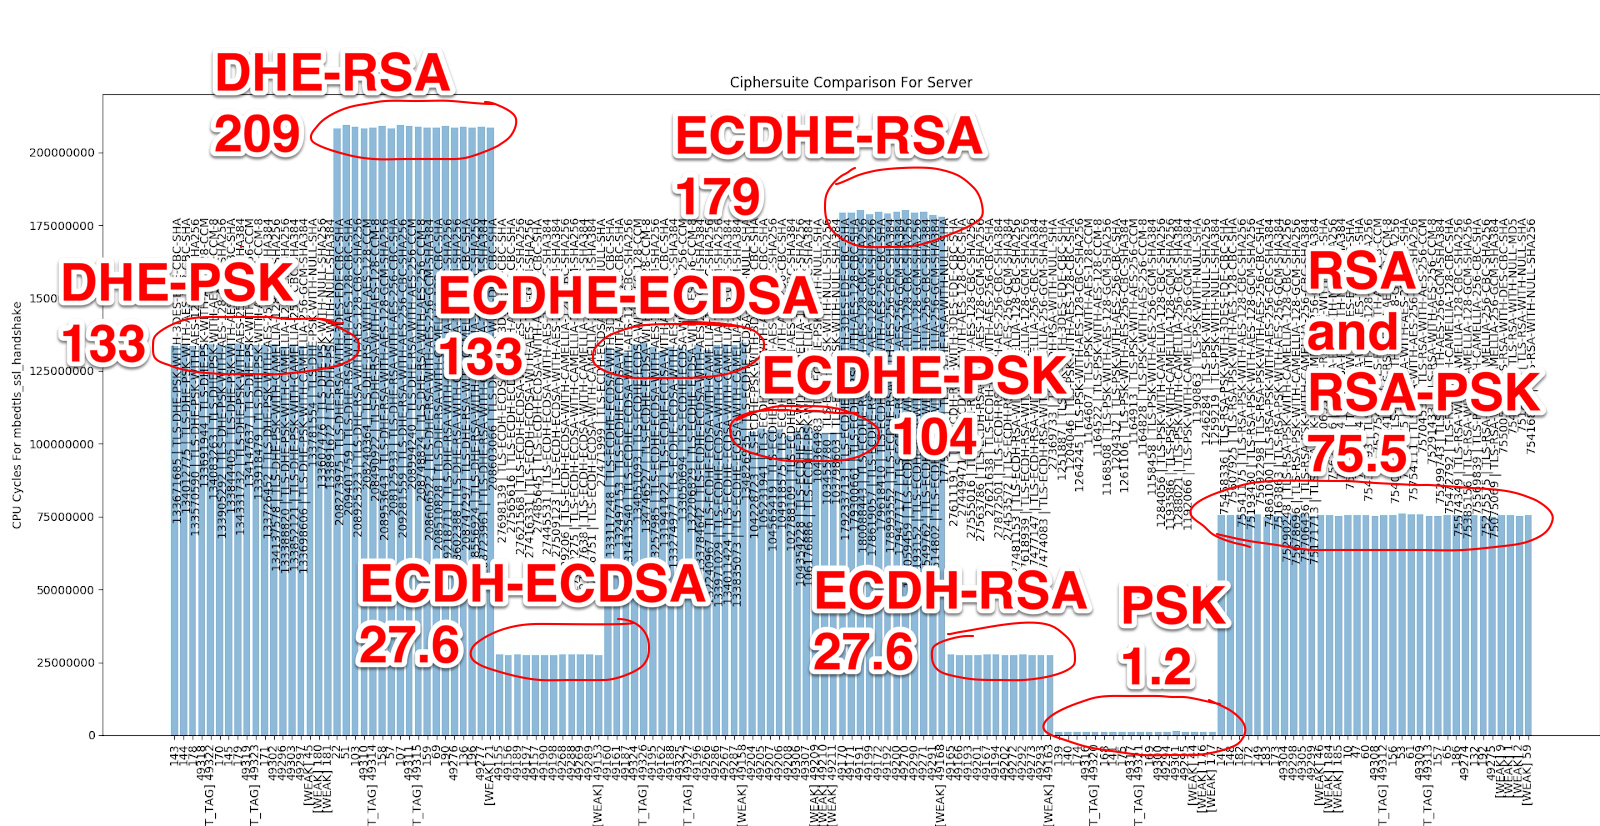
\includegraphics[width=0.5\textwidth]{./srv-graph.png} % first figure itself
        \caption{\label{fig:srvgraph} \gls{tls} Server ciphersuite profiling}
\end{figure}

The result of profiling
all of the $161$ \textit{mbedTLS} ciphersuites is presented in Figures
\ref{fig:cligraph} (for the client) and \ref{fig:srvgraph} (for the server). The various key exchange groups are identified by the letters
in red. The associated numbers refer to the approximate number of CPU
cycles (in millions) used by the ciphersuite during the handshake.

For example, Figure \ref{fig:srvgraph} shows that the server would use
$133$ million CPU cycles to perform a \gls{tls} handshake using the
\textit{ECDHE-ECDSA} ciphersuite (ephemeral ECDH with ECDSA signatures).

The comparison of the \textit{ECDHE-RSA} and \textit{ECDH-RSA}
key exchange, shows that the use of perfect forward secrecy leads to
about $6.5$ times more CPU cycles used during the handshake.

The results show different numbers for the client and the server.
This may come down to various factors, depending on the ciphersuite. In ciphersuites
that public certificates are used, during the handshake, the client needs
to verify the certificate chain provided by the server, while the
server does not. This means that the client will need to perform
public key cryptography operations, which use a lot of CPU cycles.
In the \textit{RSA} key exchange, the server encrypts a secret
and sends it to the client. The client then decerypts that secret.
Since the public exponent of the RSA keypair is usually chosen to be small (in the
case of the tested ciphersuite it's $65537$), public key operations
are much faster than private key operations. Since the client uses
the public key to decrypt the secret, while the server encrypts it
with the private key, the latter will use significantly more CPU
cycles.

Ciphersuites which do not use public key cryptography (i.e. no
certificates) show very similar results in both, the client and the server. Those ciphersuites are all of the pre-shared-key (PSK) ones, with
the exception of \textit{RSA-PSK}, which uses RSA and certificates
for authentication.

As expected, PSK ciphersuites show the best results. This is why they
are so widely used in embedded devices.

We performed similar measurements for the number of CPU cycles used
during data encryption and decryption, as well as MAC generation and verification for each one of the ciphersuites. The scenario was a $13$ MB file transfer between the client
and the server. In this case, just as expected, the majority of the
processing was spent on encrypting and encrypting the data. The handshake
became negligible.

\section{Future Work}

Throughout April 2018 the cost of each security service will be
determined more accurately. Throughout March 2018, the remaining
\gls{tls} features will be profiled and a cost associated with them.
This will help us understand which additional costs or savings
each one of them has. Throughout March and June 2018 other relevant metrics, such
as power consumption, will be collected and the the profiling
will be performed on typical \gls{iot} hardware. During this same
period, instead of using \textit{valgrind} CPU cycle estimates,
a transition to
a tool like \textit{PAPI}\cite{PAPI0:online} will be done to
obtain precise values. The automated profiling tool will be adapted accordingly. During the month of June 2018 any troubles
that arise during the previous phases will be worked on.

From June until the end of August 2018, the tool that suggests a \gls{tls}
configuration based on the environment's requirements and limitations
will be developed. It will include a Graphical User Interface.

From mid-July until mid-September 2018 the focus will be on writing
the dissertation's text.

\section{Conclusion}

The lack of security in \gls{iot} is a serious issue that can lead to a high monetary costs,
when botnets infect the devices. Recent
attacks clearly show that serious damage can be caused. An old saying attributed to the
\gls{nsa} states that "Attacks always get better; they never get worse".
Combined with the fact that the number of \gls{iot} devices is growing at a high
pace, without any major improvements to their security, makes it clear
that it is fundamental for this issue to be addressed.

While there are well established security solutions, not all of them can be used
with \gls{iot} devices, due their constrained nature. One such example is
the (D)\gls{tls} protocol, that because of its heavyweight nature is not suitable for a large part of \gls{iot} devices. With the proposed work,
we want to contribute to this area, by designing a solution that is suitable for the \gls{iot} devices, transparent
to the programmer and provides security services adaptable to the specific context needs.

\section*{Acknowledgments}

I would like to thank my supervisors, Ricardo Chaves and Aleksandar Ilic for
their continuous support, ideas and help that they have given me during
this work.

\bibliographystyle{unsrt}
\bibliography{tls_for_iot,papers}
\end{document}
